%!TEX root = ./template-skripsi.tex

\subsection{\textit{Sprint 9}}

	\textit{Sprint-9} dilakukan sepekan pada tanggal 18 oktober 2022 sampai dengan 25 oktober 2022. \textit{Story} kesembilan pada \textit{product backlog} yaitu membuat fitur pencatatan kualitas air mingguan dipecah menjadi beberapa \textit{task} sebagai berikut.


 \begin{longtable}[c]{@{} |p{1cm}|p{4cm}|p{5cm}|p{3cm}| @{}}
 \caption{\textit{Sprint 9} \label{sprint9_table}}\\


 \hline
  \multirow{1}{=}{\centering{\textbf{No}}} & \multirow{1}{=}{\centering{\textbf{\textit{Story}}}} & \multirow{1}{=}{\centering{\textbf{\textit{Task}}}} & \multirow{1}{=}{\centering{\textbf{\textit{Status}}}}\\
 \endfirsthead

 \hline
  \multirow{1}{=}{\centering{\textbf{No}}} & \multirow{1}{=}{\centering{\textbf{\textit{Story}}}} & \multirow{1}{=}{\centering{\textbf{\textit{Task}}}} & \multirow{1}{=}{\centering{\textbf{\textit{Status}}}}\\
 \endhead

 \hline
 \endfoot

 \hline
 \endlastfoot

 \hline
 1 & Membuat fitur pencatatan kualitas air mingguan &  Membuat \textit{Mock-up UI} halaman list pencatatan kualitas air mingguan, entry kualitas air mingguan, detail kualitas air mingguan  &  selesai \\
 \hline
 2 & & Menerapkan \textit{Mock-up UI} halaman list pencatatan kualitas air mingguan, entry kualitas air mingguan, detail kualitas air mingguan ke Flutter & selesai\\
 \hline
 3 & & Mengintegrasikan halaman pencatatan kualitas air mingguan, entry kualitas air mingguan, detail kualitas air mingguan ke \textit{webservice} & selesai\\
 \hline
 \end{longtable}

Pada sprint kesembilan ini story yang di pilih untuk di uraikan pada sprint kali ini adalah membuat halaman pencatatan kualitas air mingguan, entry kualitas air mingguan, detail kualitas air mingguan. Tujuan dari \textit{sprint-9} ini adalah membuat fitur pencatatan kualitas air mingguan dan mengintegrasikan halaman tersebut dengan webservice yang sudah dibuat oleh penelitian Andri Rahmanto.

\begin{enumerate}[listparindent=2em]
	
	\item{\textit{Membuat Mock-up UI Fitur Pencatatan Kualitas air mingguan}}
	
	Pembuatan konten dan fitur yang terdapat pada \textit{mock-up UI} fitur pencatatan kualitas air mingguan dilakukan berdasarkan persetujuan product owner dan scrum master pada meeting sebelumnya. Mock-up UI dibuat menggunakan platform figma.
	
	\begin{figure}[H]
	\centering
	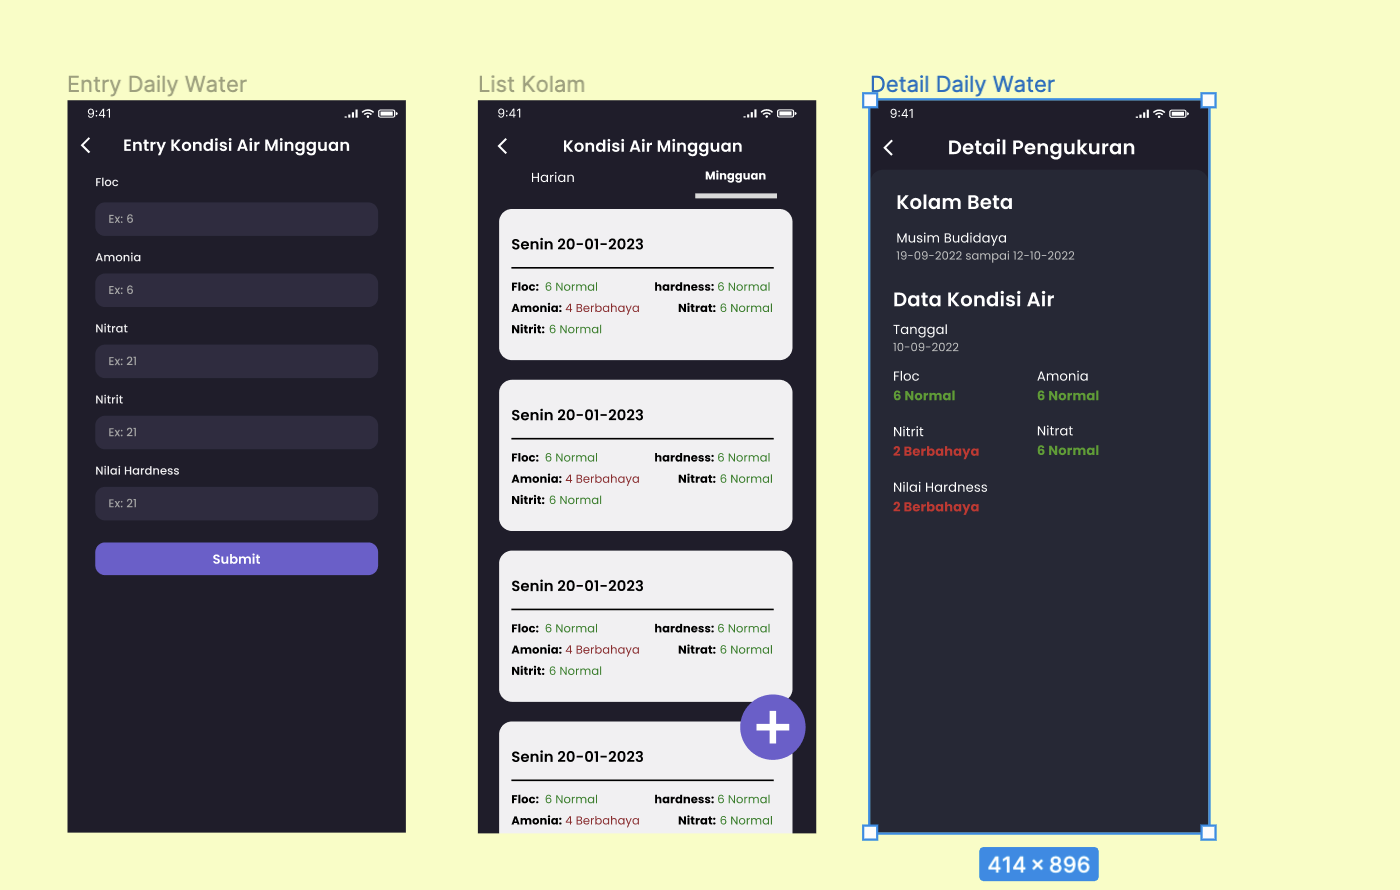
\includegraphics[keepaspectratio, width=6cm]{gambar/mockupairmingguan}
	\caption{\textit{Mock-up UI Fitur Pencatatan Kualitas air mingguan}}
	\label{gambar:mockupairmingguan}
	\end{figure}

	\item{\textit{Class Diagram}}
	
	Class Diagram menggambarkan kelas-kelas yang akan dipakai oleh sistem. Umumnya terdapat 3 kelas pada setiap module yaitu class model, controller, dan view. Pada sprint-9 penelitian kali ini penulis membuat 4 class yaitu model yang berwarna biru, view berwarna oranye, controller yang berwarna hijau, dan service yang berwarna kuning.
	 
	 \begin{figure}[H]
	 \centering
	 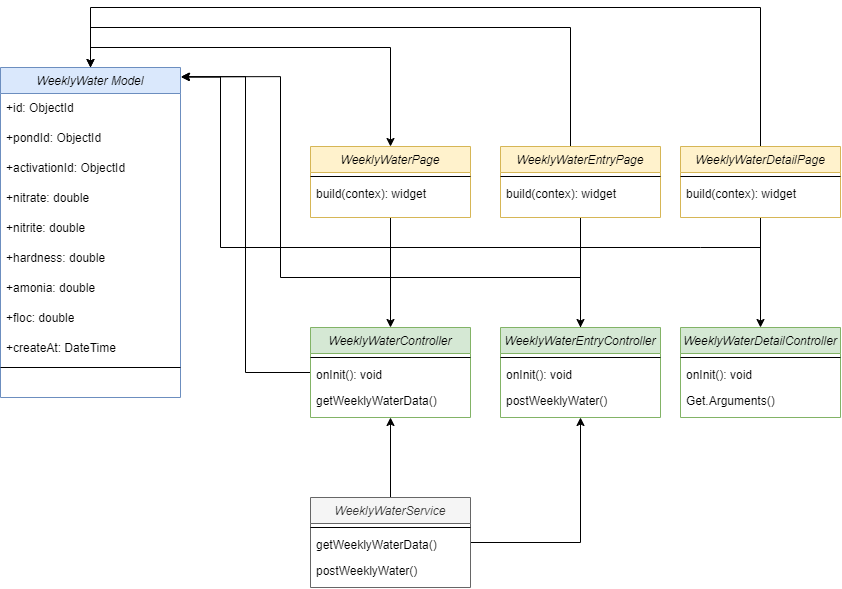
\includegraphics[keepaspectratio, width=6cm]{gambar/weeklycd}
	 \caption{\textit{Class Diagram Fitur Sprint-9}}
	 \label{gambar:weeklycd}
	 \end{figure}

	\item{\textit{Menerapkan Mockup-UI Fitur Pencatatan Kualitas air mingguan kedalam code flutter}}
	
	Setelah itu, akan dilakukan pengimplementasian \textit{mock-up UI} ke dalam aplikasi menggukan flutter. Pada lampiran 10 terdapat source code dari implementasi fitur pencatatan kualitas air mingguan yang dikelompokan berdasarkan halaman yang menghasilkan output halaman seperti dibawah ini

	\begin{figure}[H]
		\centering
		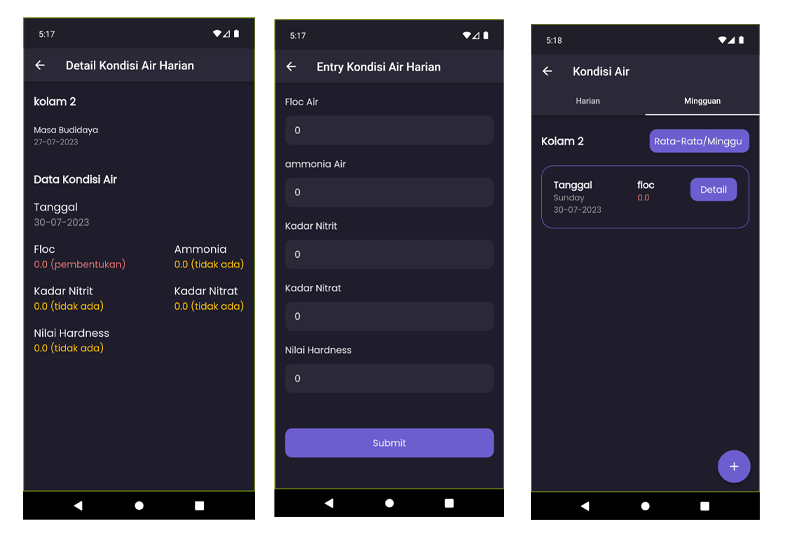
\includegraphics[keepaspectratio, width=8cm]{gambar/sssprint9}
		\caption{\textit{Output dari code pada sprint 9}}
		\label{gambar:sssprint9}
		\end{figure}

	\item{\textit{Mengitegrasikan fitur pencatatan kualitas air mingguan dengan webservice}}

	Sebelumnya, setiap data pada fitur masih berupa data dummy sehingga perlu diintegrasikan dengan webservice agar aplikasi dapat berjalan dengan data yang asli. Hal yang dilakukan dalam mengintegrasikan fitur pencatatan kualitas air mingguan dengan webservice terdapat pada lampiran 10.

  \item{Analisis \textit{User Experience}} 
 
  Pada halaman entry weekly water quality, pembudidaya harus memasukan data yang diperlukan untuk melakukan weekly water quality sesuai dengan kesepakatan saat meeting, seperti kadar nitrit, nitrat, amonia, dan nilai kekerasan air. Selain itu terdapat juga list mengenai data weekly water quality yang telah dimasukan yang berisi informasi yang berhubungan dengan weekly water quality. Terdapat pula halaman detail weekly water quality yang berisi informasi yang lebih detail terkait weekly water quality yang telah dilakukan.

\item{Sprint 9 Review dan Sprint 10 Planning}

Sprint 9 diakhiri dengan melakukan weekly meeting pada hari selasa dengan agenda melakukan review dan testing terkait hasil sprint 9 dan melakukan planning untuk sprint 10 dengan rincian:
\begin{enumerate}
	\item{\textit{Review dan Testing hasil dari sprint 9}}

	Telah dilakukan review dan testing oleh penulis selaku developer dengan Scrum Master. Setelah dilakukan testing, Scrum Master menyimpulkan bahwa fitur pencatatan kualitas air mingguan telah berjalan dengan baik.
	
  \begin{longtable}{| p{8cm} | c | c | l |}
    \caption{Unit testing Halaman Kualitas Air.\label{table:unit_testing_fitur_kualitas_air}}\\
    \hline
    \multirow{2}{*}{Skenario Pengujian} & \multicolumn{2}{l|}{Kesesuaian} & \multirow{2}{*}{Kesimpulan} \\ 
    \cline{2-3}
      & \multicolumn{1}{l|}{sesuai} & tidak sesuai & \\ 
    \hline
    \hline
    \endfirsthead
    \hline
    \multirow{2}{*}{Skenario Pengujian} & \multicolumn{2}{l|}{Kesesuaian} & \multirow{2}{*}{Kesimpulan} \\ 
    \cline{2-3}
      & \multicolumn{1}{l|}{sesuai} & tidak sesuai &  \\ 
    \hline
    \hline
    \endhead
    \hline
    \endfoot
    
    
    \hline\hline
    \endlastfoot
    Ketika memilih musim budidaya dan maka akan ditampilkan list pengontrolan kualitas air kolam & \Checkmark &  & Diterima \\ 
    \hline
    Ketika menekan list data pengontrolan kualitas air, maka akan ditamplikan detail pengontrolan kualitas air kolam & \Checkmark &  & Diterima \\ 
    \hline
    Saat ikon (+) ditekan maka akan menampilkan halaman entry pengontrolan kualitas air kolam & \Checkmark &  & Diterima \\ 
    \hline
    ketika mengisi form pengontrolan kualitas air kolam dengan data yang sesuai dan menekan submit, data pengontrolan kualitas air akan ditambahkan & \Checkmark &  & Diterima \\ 
    \hline
    \end{longtable}

	\item{\textit{Sprint Planning untuk Sprint 10}}
	
	Planning untuk sprint 10 yakni membuat fitur sortir kolam mingguan pada aplikasi \textit{Assistive Aquaculture Breeding Management}.
\end{enumerate}
\end{enumerate}